\documentclass[12pt]{article}
\usepackage[UTF8]{ctex}
\usepackage{amsmath}
\usepackage{amssymb}
\usepackage{graphicx}
\usepackage{lipsum} % 仅用于占位文本，实际使用时可删除
\usepackage{tikz}

\usetikzlibrary{positioning, arrows.meta, shapes.geometric, calc, patterns}

% 定义样式
\tikzset{
    neural/.style={circle, draw, minimum size=8mm, inner sep=0pt},
    neural-layer/.style={rectangle, draw, minimum width=10mm, minimum height=5mm, inner sep=0pt},
    chessboard/.style={line width=0.5pt, color=black!50},
    black-stone/.style={circle, fill=black, minimum size=4mm},
    white-stone/.style={circle, draw=black, fill=white, minimum size=4mm},
    arrow/.style={-{Stealth[length=4mm]}, thick},
    label/.style={font=\small, inner sep=1pt}
}

\title{Mastering the game of Go with deep 
neural networks and tree search 论文精读}
\author{Crazyfish}
\date{}

\begin{document}

\maketitle


\begin{abstract}
围棋因其巨大的搜索空间，以及评估棋盘局面和落子的困难性，长期被视为经典游戏中对人工智能最具挑战性的任务。本文提出了一种计算机围棋的新方法：
利用“价值网络”评估棋盘局面，使用“策略网络”选择落子。这些深度神经网络通过一种新颖的训练组合——从人类专家棋局中学习监督信号，
从自我对弈中学习强化信号——进行训练。在不依赖任何前瞻搜索的情况下，这些神经网络的棋力已达到最先进的蒙特卡洛树搜索程序的水平，
而后者需模拟数千局自我对弈的随机游戏。我们还提出了一种新的搜索算法，将蒙特卡洛模拟与价值、策略网络相结合。使用该算法后，
我们的程序 AlphaGo 与其他围棋程序对弈时胜率高达 $99.8\%$，并以 $5:0$ 击败了人类欧洲围棋冠军。这是计算机程序首次在全尺寸围棋游戏中战胜人类职业棋手，
而这一成就曾被认为至少需要十年才能实现。
\end{abstract}

所有完美信息博弈都存在一个最优值函数 $ v^\ast(s) $，它在所有玩家均采取完美策略的情况下，
从每一棋盘位置（或状态）$ s $ 出发，决定游戏结果。这些博弈可藉由在搜索树中递归计算最优值函数求解，
搜索树包含约 $ b^d $ 种可能行动序列，其中 $ b $ 为博弈的宽度（每位置合法行动数），$ d $ 为深度（游戏长度）。
在大型博弈中，如国际象棋（$ b\approx 35 $，$ d\approx 80 $）\cite{campbell2002deepblue}和尤其围棋
（$ b\approx 250 $，$ d\approx 150 $）\cite{schaeffer2000games}，
穷举搜索不可行\cite{allis1994searching, vandenhrik2002games}，但通过两大原则可缩减有效搜索空间。

首先，通过位置评估（position evaluation）降低搜索深度：在状态 $ s $ 处截断搜索树，
以近似值函数 $ v(s)\approx v^\ast(s) $ 替代 $ s $ 叶子树，该函数预测从 $ s $ 出发的结果。
此方法在国际象棋\cite{campbell2002deepblue}、跳棋\cite{schaeffer1992checkers}和黑白棋\cite{buro1999simple}实现超人表现，
但因围棋复杂性，人们认为其在围棋中不可行\cite{muller2002computer}。
其次，通过从策略 $ p(a|s) $ 抽样行动缩减搜索宽度，该策略为位置 $ s $ 下可能行动的概率分布。
例如，蒙特卡罗模拟\cite{tesauro1996online}搜索至最大深度不分支，在模拟（rollouts）中从策略 $ p $ 
为双方抽样长序列行动。对此类模拟取平均可提供有效局面评估，在双陆棋\cite{tesauro1996online}和拼字游戏\cite{sheppard2002scrabble}实现超人水平，
在围棋中达弱业余水平\cite{bouzy2003monte}。

蒙特卡洛树搜索（MCTS）\cite{coulom2006efficient, kocsis2006bandit}利用蒙特卡罗模拟估计搜索树各状态值。
随模拟次数增加，搜索树扩大，相关值更精确。搜索中选择行动的策略会随时间改进，通过选择值更高子节点。
渐近地，该策略收敛至完美策略，评估收敛至最优值函数\cite{kocsis2006bandit}。当前最强围棋程序基于 MCTS，
通过监督学习增强策略以预测人类专家行动\cite{coulom2007computing}。此策略用于将搜索限制在高概率行动束中，
并在模拟中抽样行动。该方法实现强业余水平\cite{coulom2007computing, baudis2012pachi, muller2010fuego}。
然而，先前工作仅限于基于输入特征线性组合的浅层策略或值函数\cite{gelly2007combining}。

近期，深度卷积神经网络在视觉领域取得空前性能：如图像分类\cite{krizhevsky2012imagenet}、
人類性别识别\cite{lawrence1997face}和玩 Atari 游戏\cite{mnih2015human}。它们使用多层神经元，
每层以重叠块排列，构建图像逐层抽象局部表示\cite{lecun2015deep}。我们为围棋采用类似架构：将棋盘位置作 $19\times19$ 图像输入，
用卷积层构建位置表示。我们利用神经网络缩减搜索树有效深度与宽度：用值网络评估局面，用策略网络抽样行动。

我们采用含多阶段机器学习的管道训练神经网络（图1）。
首先，直接从人类专家行动训练监督学习（SL）策略网络 $ p_\sigma $，
提供快速高效学习更新、即时反馈与高质量梯度。类似先前工作\cite{coulom2007computing, muller2010fuego}，
我们还训练快速策略 $ p_\pi $，能在模拟中快速抽样行动。接着，训练强化学习（RL）策略网络 $ p_\rho $，
通过自我博弈最终结果优化 SL 策略网络，将策略调整至正确胜利目标，而非最大化预测准确性。
最后，训练值网络 $ v_\theta $ 预测 RL 策略网络自我博弈结果。我们的程序 AlphaGo 高效结合策略与值网络和 MCTS。

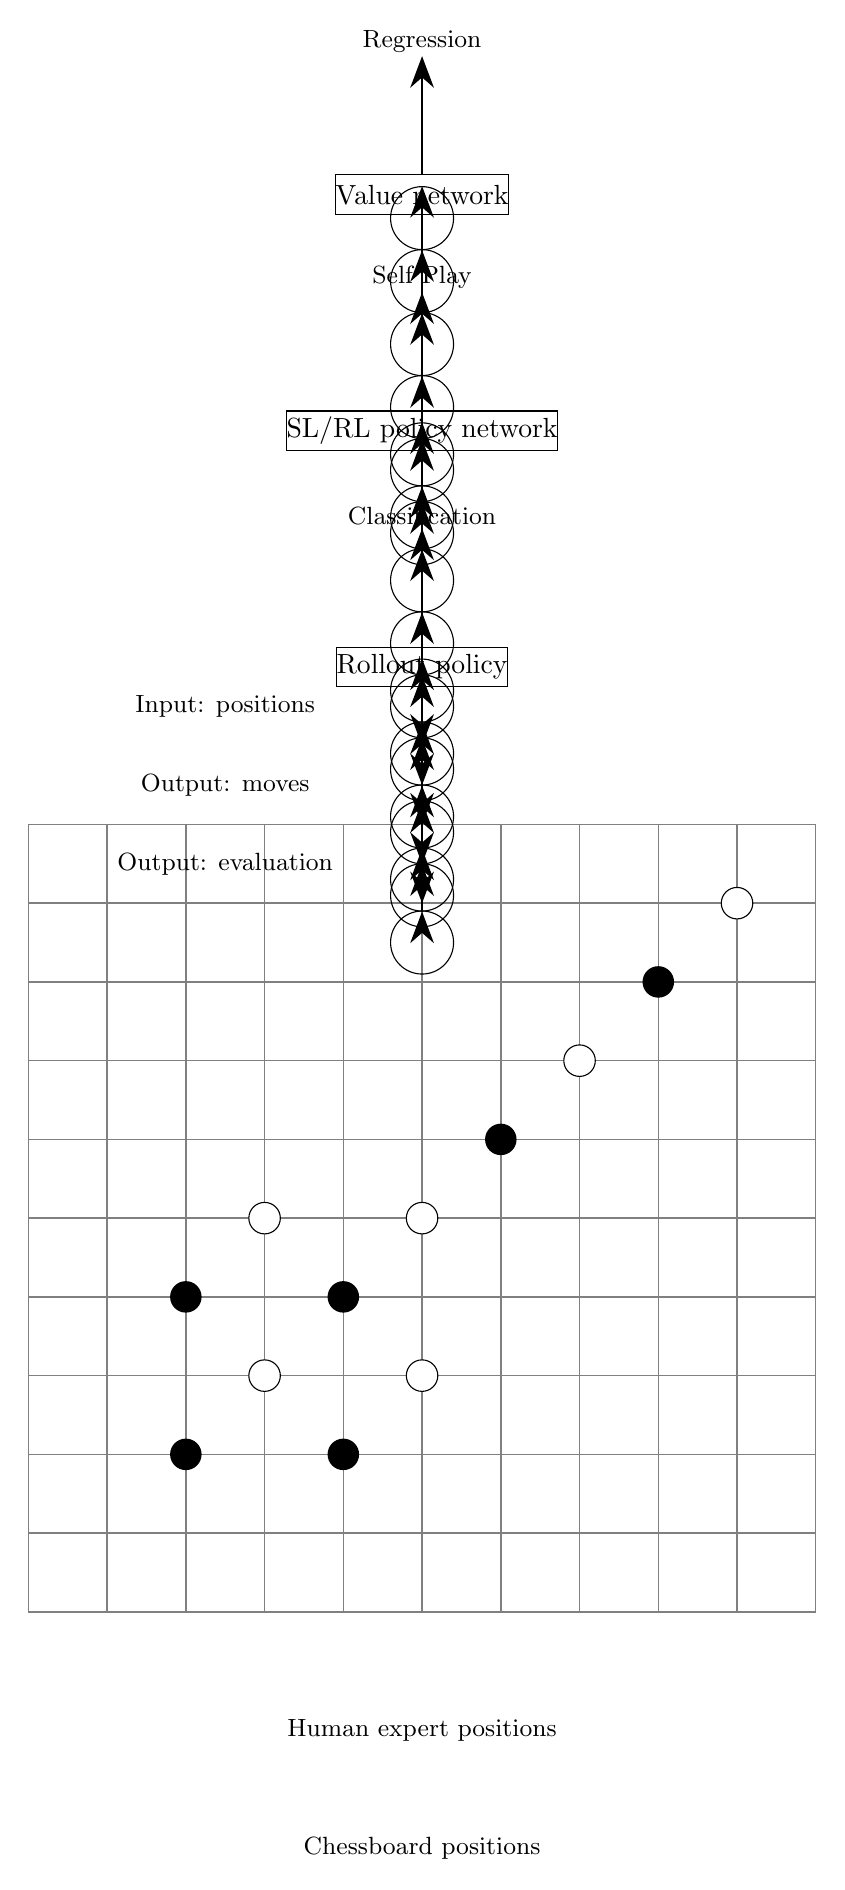
\begin{tikzpicture}[node distance=12mm and 8mm]

% 绘制棋盘
\draw[chessboard] (0,0) grid (10,10);
\foreach \x in {0,1,...,10} {
    \draw[chessboard] (\x,0) -- (\x,10);
    \draw[chessboard] (0,\x) -- (10,\x);
}

% 添加棋子（示例位置）
\foreach \x/\y in {2/2, 2/4, 4/2, 4/4, 6/6, 8/8} {
    \node[black-stone] at (\x,\y) {};
}
\foreach \x/\y in {3/3, 3/5, 5/3, 5/5, 7/7, 9/9} {
    \node[white-stone] at (\x,\y) {};
}

% 添加棋盘标签
\node[label] at (5,-1.5) {Human expert positions};
\node[label] at (5,-3) {Chessboard positions};

% 绘制神经网络：Rollout policy
\node[neural-layer] (rollout) at (5, 12) {Rollout policy};
\foreach \i in {1,...,5} {
    \node[neural] (r\i) at (5, 12.5-\i*0.8) {};
}
\draw[arrow] (rollout.south) -- (r1.north);
\foreach \i [count=\j from 1] in {1,...,4} {
    \draw[arrow] (r\i) -- (r\j.south);
}

% 绘制神经网络：SL/RL policy network
\node[neural-layer] (policy) at (5, 15) {SL/RL policy network};
\foreach \i in {1,...,8} {
    \node[neural] (p\i) at (5, 15.5-\i*0.8) {};
}
\draw[arrow] (policy.south) -- (p1.north);
\foreach \i [count=\j from 1] in {1,...,7} {
    \draw[arrow] (p\i) -- (p\j.south);
}

% 绘制神经网络：Value network
\node[neural-layer] (value) at (5, 18) {Value network};
\foreach \i in {1,...,6} {
    \node[neural] (v\i) at (5, 18.5-\i*0.8) {};
}
\draw[arrow] (value.south) -- (v1.north);
\foreach \i [count=\j from 1] in {1,...,5} {
    \draw[arrow] (v\i) -- (v\j.south);
}

% 添加标注箭头
\draw[arrow] (rollout.north) -- ++(0,1.5) node[label, above] {Classification};
\draw[arrow] (policy.north) -- ++(0,1.5) node[label, above] {Self Play};
\draw[arrow] (value.north) -- ++(0,1.5) node[label, above] {Regression};

% 添加棋盘与神经网络的连接
\draw[arrow] (rollout.south) -- (5,11);
\draw[arrow] (policy.south) -- (5,10);
\draw[arrow] (value.south) -- (5,9);

% 添加数据流标注
\node[label] at (2.5, 11.5) {Input: positions};
\node[label] at (2.5, 10.5) {Output: moves};
\node[label] at (2.5, 9.5) {Output: evaluation};

% 添加数据流箭头
\draw[arrow] (5,11) -- (5,10.5);
\draw[arrow] (5,10) -- (5,9.5);

\end{tikzpicture}


\bibliographystyle{plain}
\bibliography{refs}

\end{document}